%%%%%%%%%%%%%%%%%%%%%%%%%%%%%%%%%%%%%%%%%
% Beamer Presentation
% LaTeX Template
% Version 1.0 (10/11/12)
%
% This template has been downloaded from:
% http://www.LaTeXTemplates.com
%
% License:
% CC BY-NC-SA 3.0 (http://creativecommons.org/licenses/by-nc-sa/3.0/)
%
%%%%%%%%%%%%%%%%%%%%%%%%%%%%%%%%%%%%%%%%%

%----------------------------------------------------------------------------------------
%	PACKAGES AND THEMES
%----------------------------------------------------------------------------------------

\documentclass{beamer}

%% \mode<presentation> {

% The Beamer class comes with a number of default slide themes
% which change the colors and layouts of slides. Below this is a list
% of all the themes, uncomment each in turn to see what they look like.

%\usetheme{default}
%\usetheme{AnnArbor}
%\usetheme{Antibes}
%\usetheme{Bergen}
%\usetheme{Berkeley}
%\usetheme{Berlin}
%\usetheme{Boadilla}
%\usetheme{CambridgeUS}
%\usetheme{Copenhagen}
%\usetheme{Darmstadt}
%\usetheme{Dresden}
%\usetheme{Frankfurt}
%\usetheme{Goettingen}
%\usetheme{Hannover}
%\usetheme{Ilmenau}
%\usetheme{JuanLesPins}
%\usetheme{Luebeck}
\usetheme{Madrid}
%% \usetheme{Malmoe}
%\usetheme{Marburg}
%\usetheme{Montpellier}
%% \usetheme{PaloAlto}
%\usetheme{Pittsburgh}
%\usetheme{Rochester}
%\usetheme{Singapore}
%\usetheme{Szeged}
%% \usetheme{Warsaw}

% As well as themes, the Beamer class has a number of color themes
% for any slide theme. Uncomment each of these in turn to see how it
% changes the colors of your current slide theme.

%\usecolortheme{albatross}
%\usecolortheme{beaver}
%\usecolortheme{beetle}
%\usecolortheme{crane}
%\usecolortheme{dolphin}
%\usecolortheme{dove}
%\usecolortheme{fly}
%\usecolortheme{lily}
%\usecolortheme{orchid}
%\usecolortheme{rose}
%\usecolortheme{seagull}
%\usecolortheme{seahorse}
%\usecolortheme{whale}
%\usecolortheme{wolverine}

%\setbeamertemplate{footline} % To remove the footer line in all slides uncomment this line
%% \setbeamertemplate{footline}[page number] % To replace the footer line in all slides with a simple slide count uncomment this line

\setbeamertemplate{navigation symbols}{} % To remove the navigation symbols from the bottom of all slides uncomment this line
%% }

\usepackage[T2A]{fontenc}
\usepackage[utf8]{inputenc}
\usepackage[english,russian]{babel}
\usepackage[style=authoryear]{biblatex} 
\usepackage{graphicx} % Allows including images
\usepackage{booktabs} % Allows the use of \toprule, \midrule and \bottomrule in tables
\usepackage{appendixnumberbeamer}

\DeclareMathOperator{\argmin}{argmin}
\DeclareMathOperator{\argmax}{argmax}

%----------------------------------------------------------------------------------------
%	TITLE PAGE
%----------------------------------------------------------------------------------------

% The short title appears at the bottom of every slide, the full title is only on the title page
\title[DQN-routing]{Глубокие самообучающиеся агенты в мультиагентной системе маршрутизации} 

\author[Дмитрий Мухутдинов, М3438]{
    Мухутдинов Дмитрий, группа M3438 \\
    Научный руководитель: Фильченков А. А., к.ф-м.н., доцент кафедры КТ \\
    Рецензент: Тарасов В. Б., к.т.н., МГТУ им. Баумана
}% Your name
\institute[ИТМО] % Your institution as it will appear on the bottom of every slide, may be shorthand to save space
{
    Кафедра Компьютерных Технологий \\
    Факультет Информационных Технологий и Программирования \\
    Университет ИТМО, Санкт-Петербург
}
\date{\today} % Date, can be changed to a custom date

\graphicspath{{img/}}

\begin{document}

\frame{\titlepage}

%----------------------------------------------------------------------------------------
%	PRESENTATION SLIDES
%----------------------------------------------------------------------------------------

\section{First Section} 

\subsection{Subsection Example} % A subsection can be created just before a set of slides with a common theme to further break down your presentation into chunks

\begin{frame}
  \frametitle{Задача маршрутизации}
  \begin{itemize}
  \item Сетевой роутинг
  \item Транспортная логистика
  \item Управление конвейерными системами
  \item Автоматическое управление городским трафиком
  \item ...
  \end{itemize}
\end{frame}

%------------------------------------------------

\begin{frame}
  \frametitle{Существующие решения}
  \begin{itemize}
  \item Link-state
    \begin{itemize}
    \item Open Shortest Path First (OSPF)
    \item IS-IS
    \end{itemize}
  \item Distance-vector
    \begin{itemize}
    \item RIP
    \item IGRP
    \end{itemize}
  \item Прочие
    \begin{itemize}
    \item AntNet
    \item ...
    \end{itemize}
  \end{itemize}
\end{frame}

%------------------------------------------------

\begin{frame}
  \frametitle{Цель работы}
  \begin{itemize}
  \item Примерно все алгоритмы маршрутизации заточены под компьютерные сети
  \item В других задачах существуют свои, более сложные условия
    \begin{itemize}
    \item Скорую нужно пропустить сквозь пробку, а обычный автомобиль --- нет
    \item Хочется минимизировать энергопотребление конвейеров
    \item ...
    \end{itemize}
  \item Задача: построить алгоритм, способный адаптироваться под гетерогенные условия
  \end{itemize}
\end{frame}

%------------------------------------------------

%% \begin{frame}
%%   \frametitle{Задача}
%%   \center{Построить алгоритм, способный адаптироваться под гетерогенные условия}
%% \end{frame}

%------------------------------------------------

\begin{frame}
  \frametitle{Идея}
  \begin{itemize}
  \item Обучение с подкреплением
  \item Нейросети в качестве обучающихся агентов
  \item Q-routing (Boyan \& Littman, 1994)
    \begin{itemize}
    \item Не получил широкого распространения в компьютерных сетях (использует
      слишком много служебных пакетов)
    \item В других задачах (трафик, конвейеры) это не является проблемой.
    \end{itemize}
  \end{itemize}
\end{frame}

%------------------------------------------------

\begin{frame}
  \frametitle{Постановка задачи в терминах RL}
  \begin{itemize}
    \item Рассмотрим \textit{пакет} в сети как обучающегося агента,
      взаимодействующего с сетью как со средой
    \item Полное состояние среды неизвестно, состояние текущего роутера ---
      \textit{наблюдение} пакета
    \item Действие --- переход к одному из соседей
    \item Q-learning:
      \[
      Q(o_t, a_t) \leftarrow r_t + \gamma \cdot
      \max\limits_{a \in \mathcal{A}_{o_{t+1}}} {Q(o_{t+1}, a)}
      \]
    \item Принцип аналогичный Q-routing:
      \[
      Q_x(d, y) \leftarrow (t_{finish} - t_{start}) +
      \max\limits_{z \in \{ V | (y, z) \in E\}} {Q_y(d, z)}
      \]
  \end{itemize}
\end{frame}

%-------------------------------------------------

\begin{frame}
  \frametitle{Базовая архитектура нейросети}
  Вход нейросети $o = (d, n, y_1 ... y_n, o')$, где:
  \begin{itemize}
  \item $d$ --- узел назначения, $n$ --- текущий узел, $y_1 ... y_n$ --- номера
    соседей, $o'$ --- любая дополнительная информация
  \item Выходы нейросети $a_1 ... a_n$ --- оценки $Q(o, a)$ для всех узлов сети
    ($-\infty$ для узлов, не являющихся соседями)
  \item Кодируем номера унитарным кодом, чтобы избежать корреляции результатов
  \item Используем RMSProp для оптимизации
  \end{itemize}
\end{frame}

%--------------------------------------------------

\begin{frame}
  \frametitle{Варианты архитектуры нейросети}
  \fontsize{6pt}{7.2}\selectfont
  \begin{columns}
    \begin{column}{0.3\textwidth}
      Feed-forward
      \begin{center}
        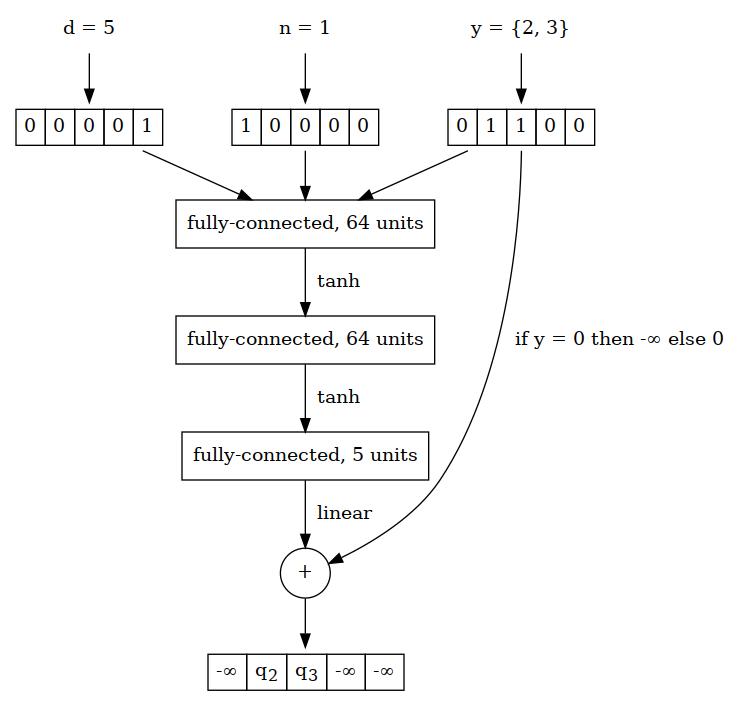
\includegraphics[width=\textwidth]{nn-1}
      \end{center}
    \end{column}
    \begin{column}{0.3\textwidth}
      LSTM с ``памятью роутера''
      \begin{center}
        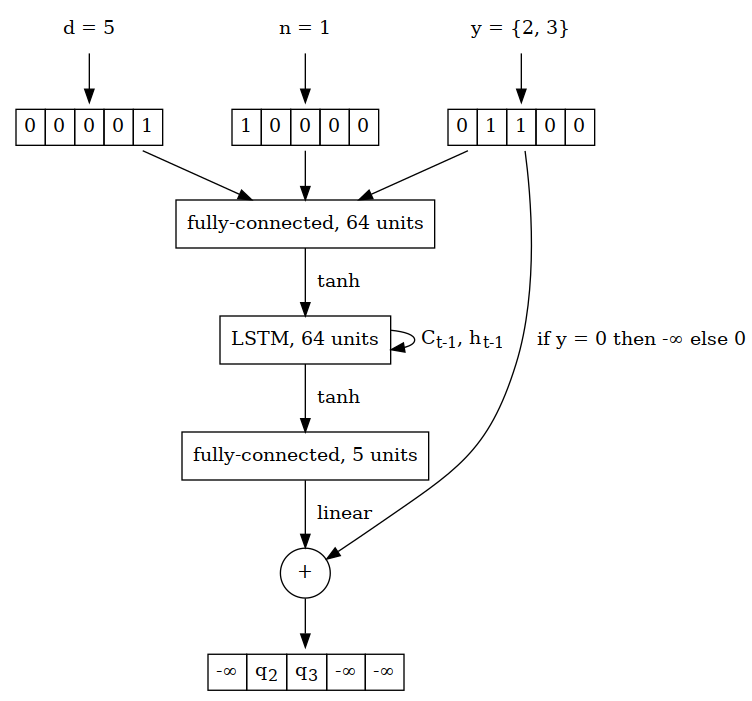
\includegraphics[width=\textwidth]{nn-3}
      \end{center}
    \end{column}
    \begin{column}{0.3\textwidth}
      LSTM c ``памятью пакета''
      \begin{center}
        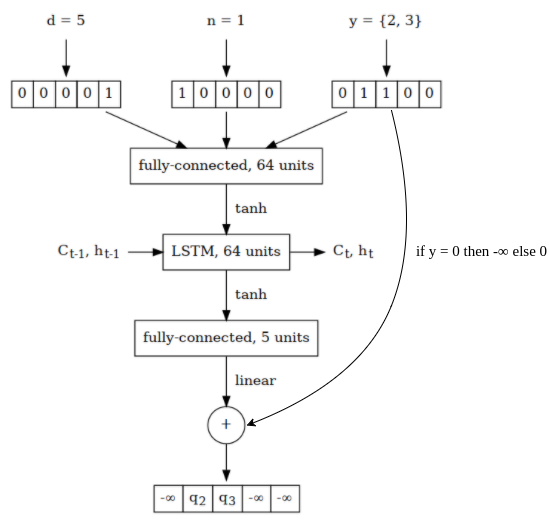
\includegraphics[width=\textwidth]{nn-4-final}
      \end{center}
    \end{column}
  \end{columns}
\end{frame}

%---------------------------------------------------

\begin{frame}
  \frametitle{Проблема нестационарности}
  \begin{itemize}
    \item Q-обучение, вообще говоря, не сходится к оптимальному решению в случае
      бесконечного числа состояний
    \item Другие агенты меняют свое поведение --- среда нестационарна,
      вследствие чего experience replay (Mnih et al., 2015) не работает
    \item При обучении с нуля на равномерной низкой нагрузке нейросети не могут
      найти оптимальные пути
  \end{itemize}
\end{frame}

%---------------------------------------------------

%---------------------------------------------------

\begin{frame}
  \frametitle{Решение проблемы нестационарности}
  \begin{itemize}
  \item Предобучение сети (bootstrapping)
    \begin{itemize}
      \item Собираем данные работы алгоритма кратчайших путей
      \item Обучаем одну нейросеть на данных от всех роутеров
      \item Предобученная сеть повторяет работу алгоритма кратчайших путей
    \end{itemize}
  \item Отказ от experience replay во время работы
    \begin{itemize}
    \item Условия работы в сети меняются
    \item Старый опыт перестает быть актуальным
    \item Если обращать на него внимание, адаптивность к изменяющимся условиям страдает
    \end{itemize}
  \end{itemize}
\end{frame}

%---------------------------------------------------

\begin{frame}
  \frametitle{Расширение наблюдаемого состояния}
  \begin{columns}
    \begin{column}{0.5\textwidth}
      Добавим на вход дополнительную информацию
      \begin{itemize}
      \item Топологию сети полезно учитывать
      \item Используем link-state протокол для обновления информации о топологии
      \item Подаем матрицу смежности графа на вход
      \end{itemize}
    \end{column}
    \begin{column}{0.5\textwidth}
      \begin{center}
        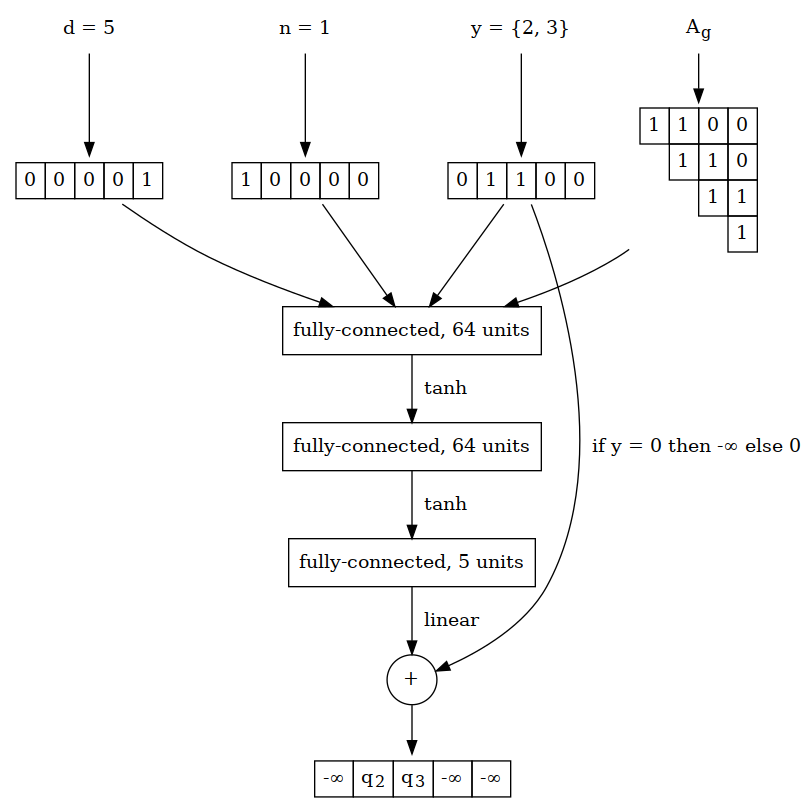
\includegraphics[width=\textwidth]{nn-2}
      \end{center}
    \end{column}
  \end{columns}
\end{frame}

%-----------------------------------------------------

\begin{frame}
  \frametitle{Компромисс между исследованием и использованием}
  \begin{itemize}
  \item Алгоритм может застревать в локальном максимуме
  \item Сложности с возвращением к оптимальной стратегии после изменений условий среды
  \item Решение: используем softmax-стратегию, чтобы иметь шанс выбрать не максимально ``выгодное'' действие:
    \[
    \sigma(z)_j = \frac{e^{z_j}}{\sum_{k=1}^K {e^{z_k}}} \; \; \mathrm{for} \; \; j
    = 1 \; .. \; K
    \]
    \[
    P(a \; | \; o) = \sigma(Q(o, a)) 
    \]
  \end{itemize}
\end{frame}

%-----------------------------------------------------

\begin{frame}
  \frametitle{Эксперименты в модели компьютерной сети}
  \begin{columns}
    \begin{column}{0.6\textwidth}
      \begin{itemize}
      \item Запуск экспериментов в симуляторе
      \item Сравнение архитектур между собой и сравнение с алгоритмами link-state и Q-routing
      \item Служебные сообщения доставляются бесплатно
      \end{itemize}
    \end{column}
    \begin{column}{0.4\textwidth}
      \begin{center}
        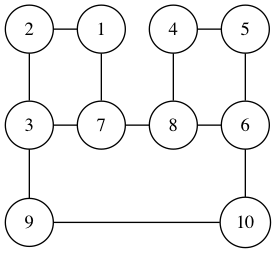
\includegraphics[width=0.7\textwidth]{graph-2}

        Топология сети для тестов
      \end{center}
    \end{column}
  \end{columns}
\end{frame}

%------------------------------------------------------

\begin{frame}
  \frametitle{Изменение топологии сети: сравнение архитектур нейросетей}
  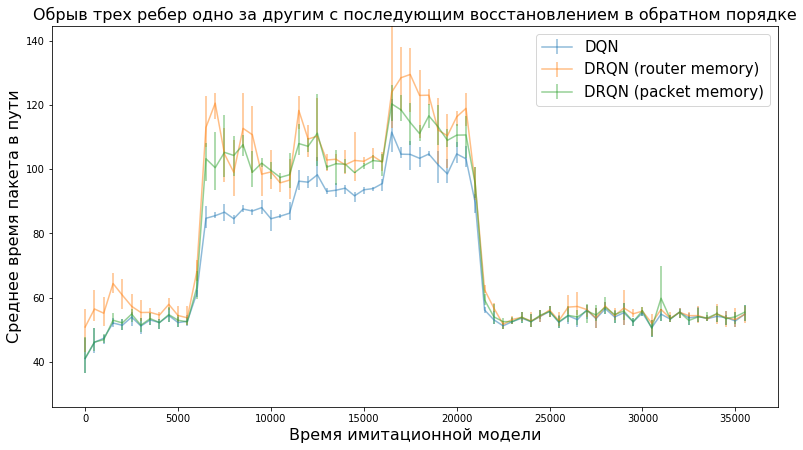
\includegraphics[width=\textwidth]{experiment-link-failures-networks} 
\end{frame}

%------------------------------------------------------

\begin{frame}
  \frametitle{Изменение топологии сети: сравнение с link-state и Q-routing}
  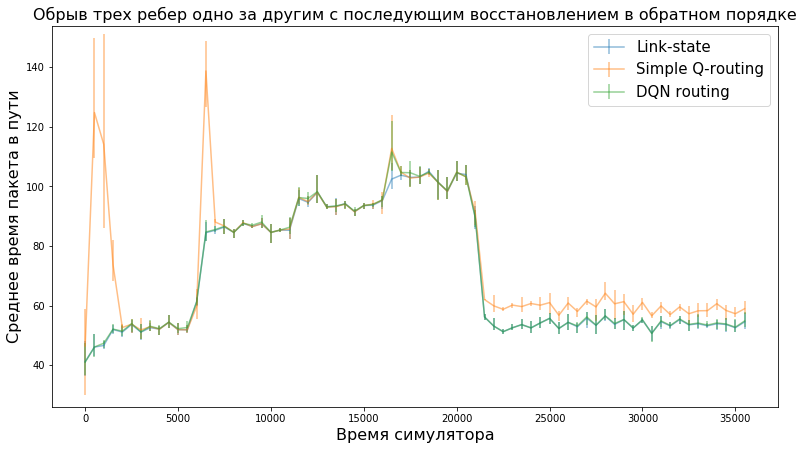
\includegraphics[width=\textwidth]{experiment-link-failures} 
\end{frame}

%------------------------------------------------------

\begin{frame}
  \frametitle{Изменение нагрузки: сравнение архитектур нейросетей}
  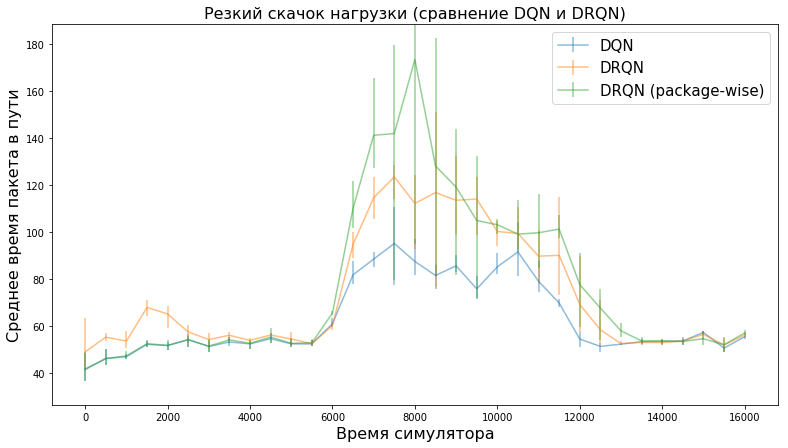
\includegraphics[width=\textwidth]{experiment-rnn-comparison} 
\end{frame}

%------------------------------------------------------

\begin{frame}
  \frametitle{Изменение нагрузки: сравнение c link-state и Q-routing}
  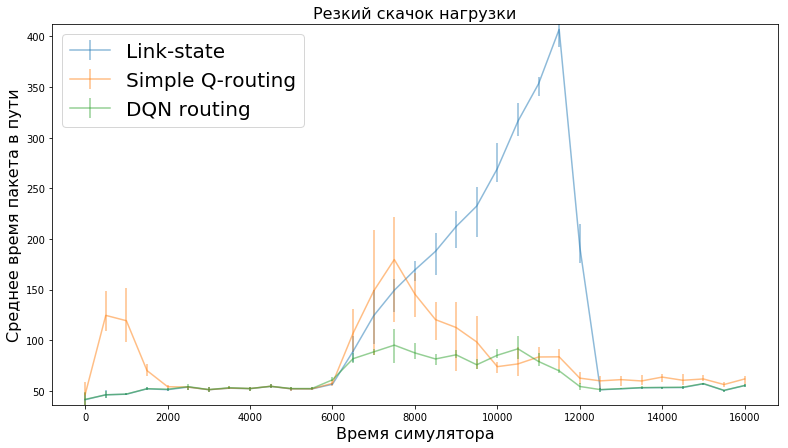
\includegraphics[width=\textwidth]{experiment-peak-load} 
\end{frame}

%------------------------------------------------------

\begin{frame}
  \frametitle{Эксперименты в модели системы багажных конвейеров}
  \begin{columns}
    \begin{column}{0.5\textwidth} 
      \begin{itemize}
      \item Конвейерная сеть моделируется как ориентированный граф
      \item Каждая секция конвейера -- отдельная вершина
      \item В оптизируемую функцию включено \textit{энергопотребление}
      \item На вход нейросети дополнительно подается информация о состоянии конвейеров
      \item Важность экономии энергии регулируется параметром $\alpha$
      \end{itemize}
    \end{column}
    \begin{column}{0.5\textwidth}
      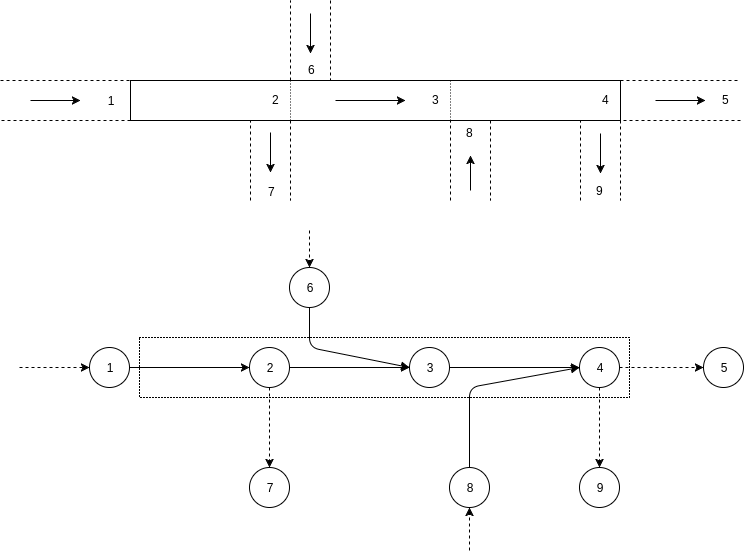
\includegraphics[width=\textwidth]{belt-illustration}  

      Участок конвейерной сети и соответствующий участок графа
    \end{column}
  \end{columns}
\end{frame}

%------------------------------------------------------

\begin{frame}
  \frametitle{Модель конвейерной системы для проведения экспериментов}
  \begin{center}
    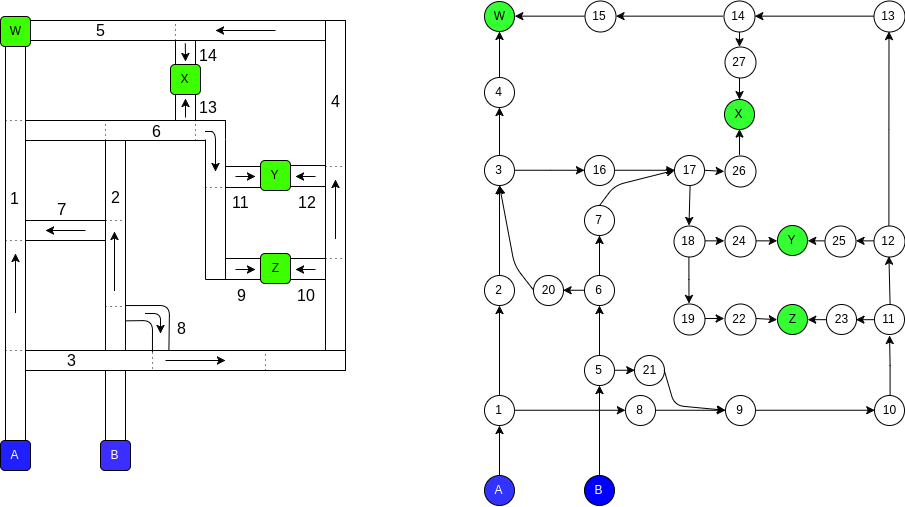
\includegraphics[width=0.9\textwidth]{test-conveyors} 
  \end{center}
\end{frame}

%------------------------------------------------------

\begin{frame}
  \frametitle{Неравномерный поток до выходных вершин: сравнение архитектур нейросетей}
  \begin{columns}
    \begin{column}{0.5\textwidth}
      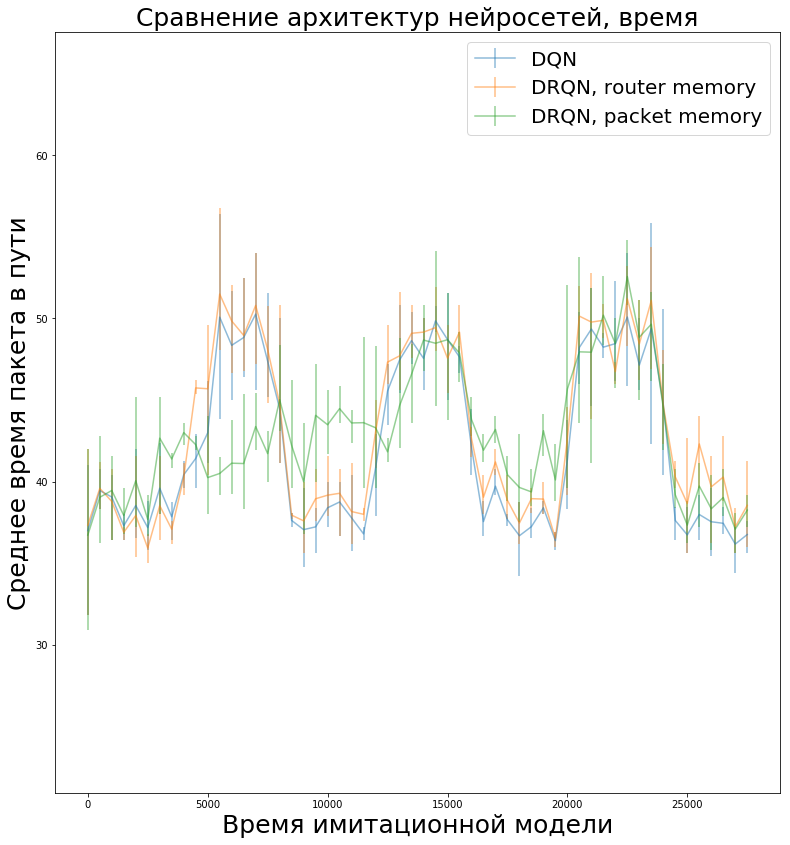
\includegraphics[width=\textwidth]{experiment-conveyors-en1-time-nns-tall}
    \end{column}
    \begin{column}{0.5\textwidth}
      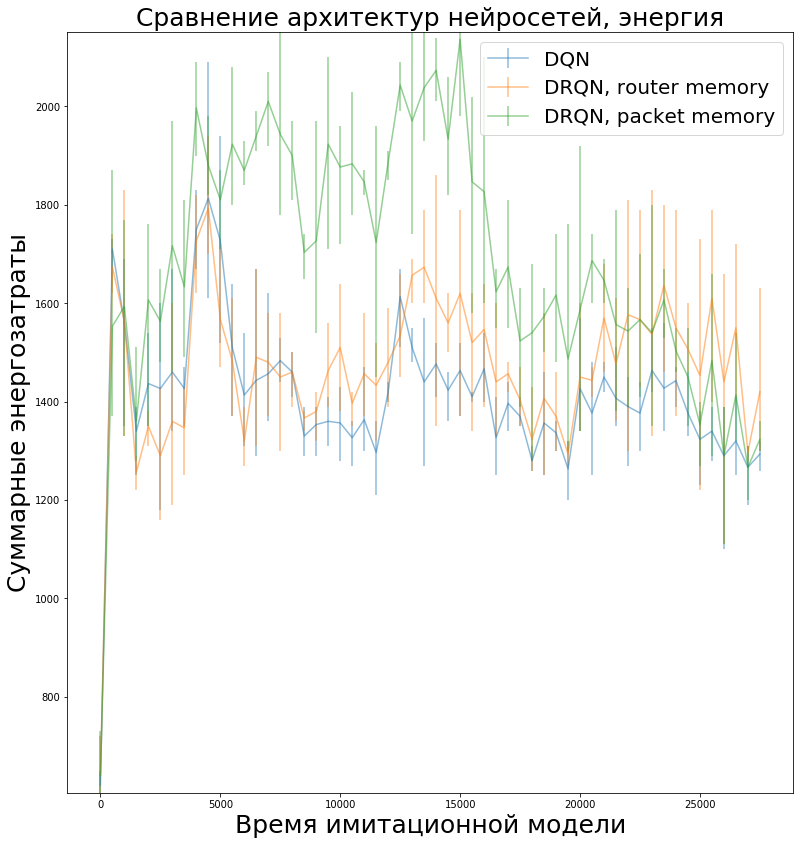
\includegraphics[width=\textwidth]{experiment-conveyors-en1-energy-nns-tall}
    \end{column}
  \end{columns}
\end{frame}

%------------------------------------------------------

\begin{frame}
  \frametitle{Неравномерный поток до выходных вершин: сравнение c link-state и Q-routing}
  \begin{columns}
    \begin{column}{0.5\textwidth}
      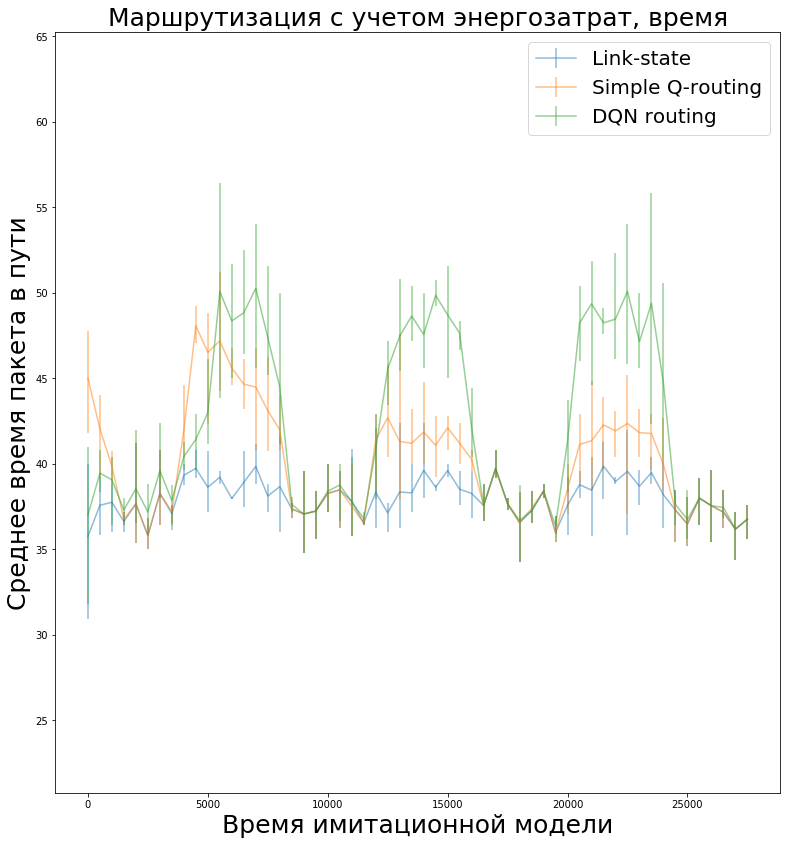
\includegraphics[width=\textwidth]{experiment-conveyors-en1-time-tall}
    \end{column}
    \begin{column}{0.5\textwidth}
      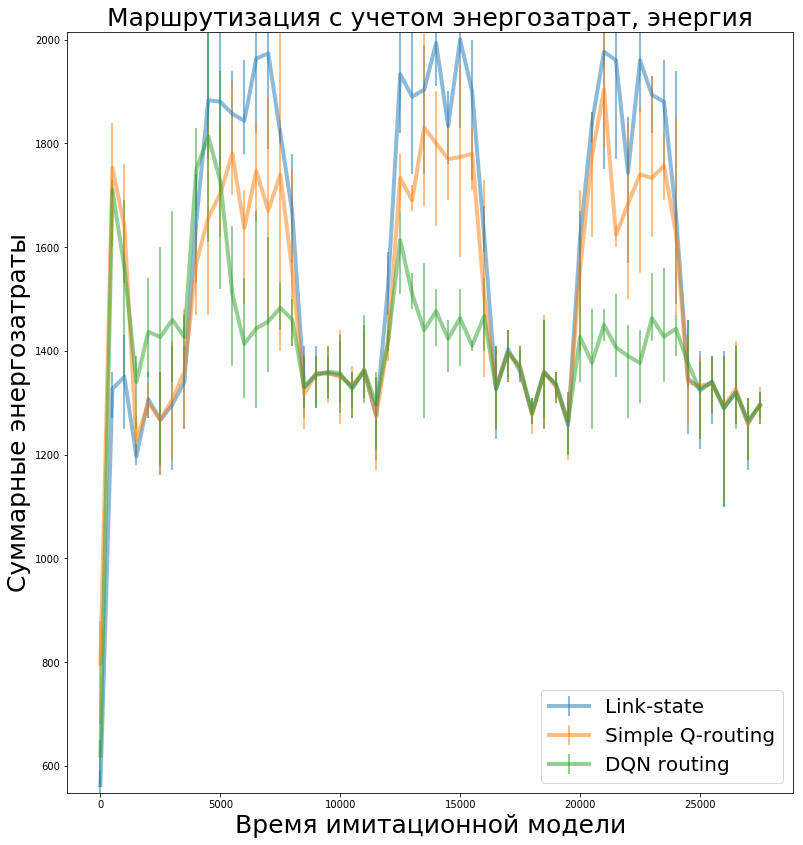
\includegraphics[width=\textwidth]{experiment-conveyors-en1-energy-tall}
    \end{column}
  \end{columns}
\end{frame}

%------------------------------------------------------

\begin{frame}
  \frametitle{Плавное повышение нагрузки: $\alpha = 1$}
  \begin{columns}
    \begin{column}{0.5\textwidth}
      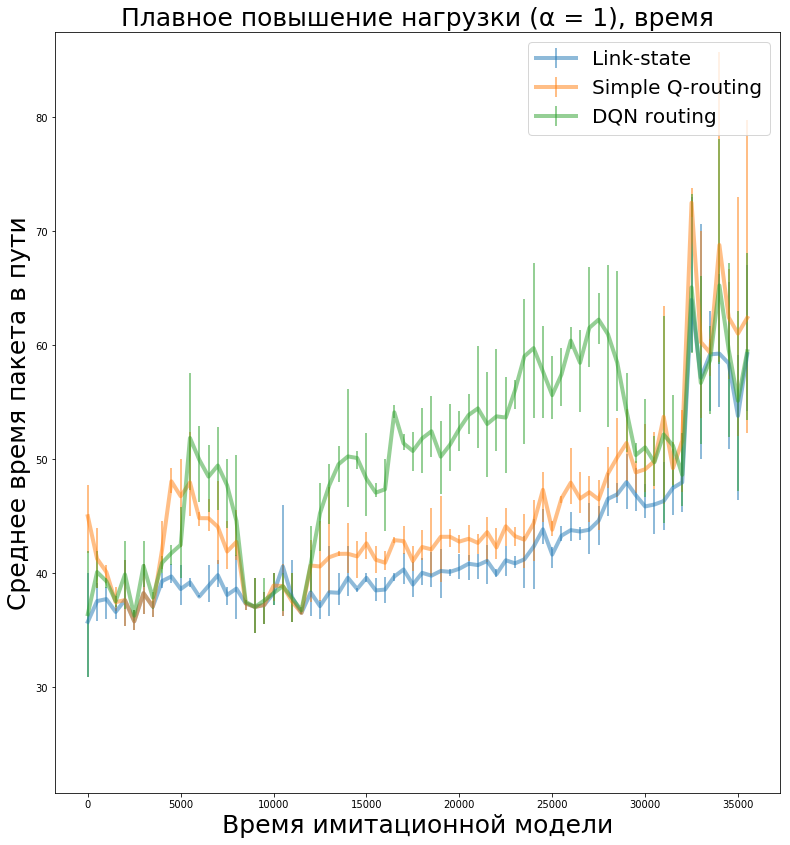
\includegraphics[width=\textwidth]{experiment-conveyors-a1-time-tall}
    \end{column}
    \begin{column}{0.5\textwidth}
      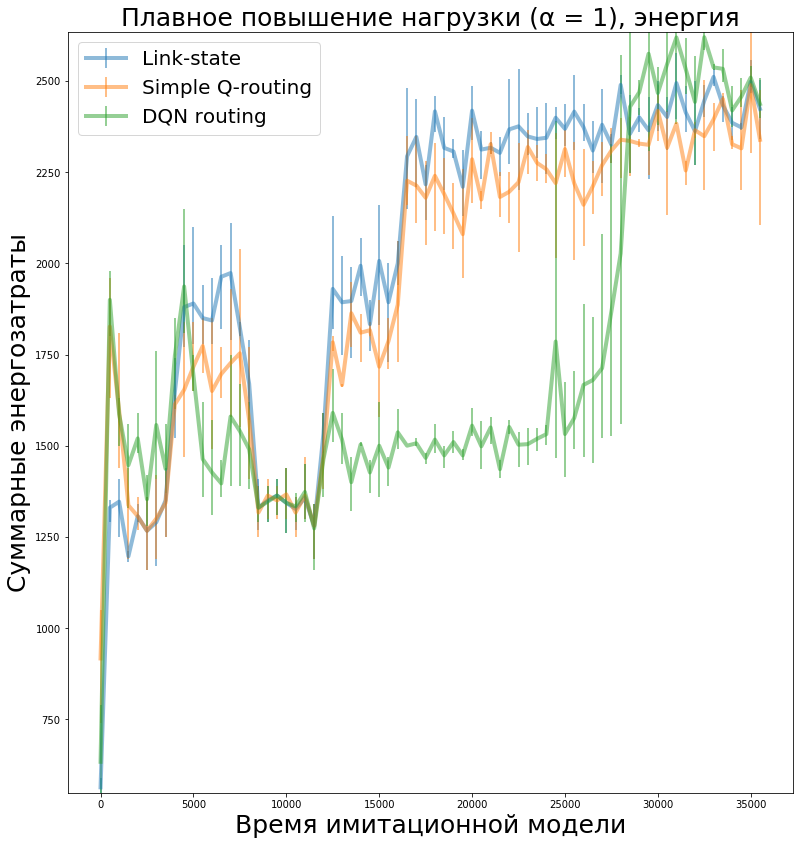
\includegraphics[width=\textwidth]{experiment-conveyors-a1-energy-tall}
    \end{column}
  \end{columns}
\end{frame}

%------------------------------------------------------

\begin{frame}
  \frametitle{Плавное повышение нагрузки: $\alpha = 0.6$}
  \begin{columns}
    \begin{column}{0.5\textwidth}
      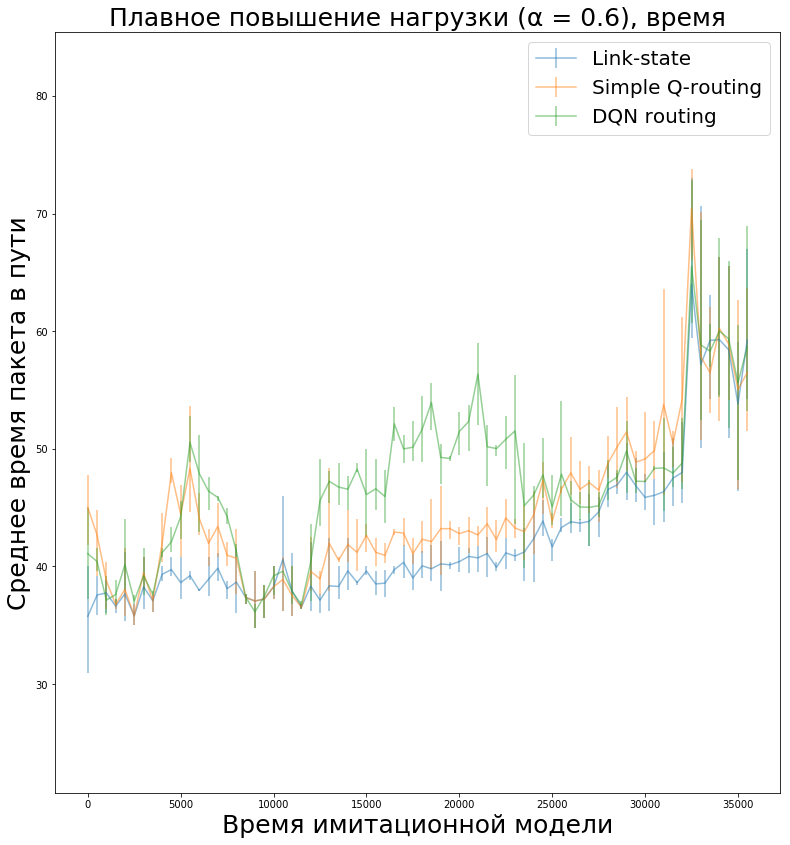
\includegraphics[width=\textwidth]{experiment-conveyors-a06-time-tall}
    \end{column}
    \begin{column}{0.5\textwidth}
      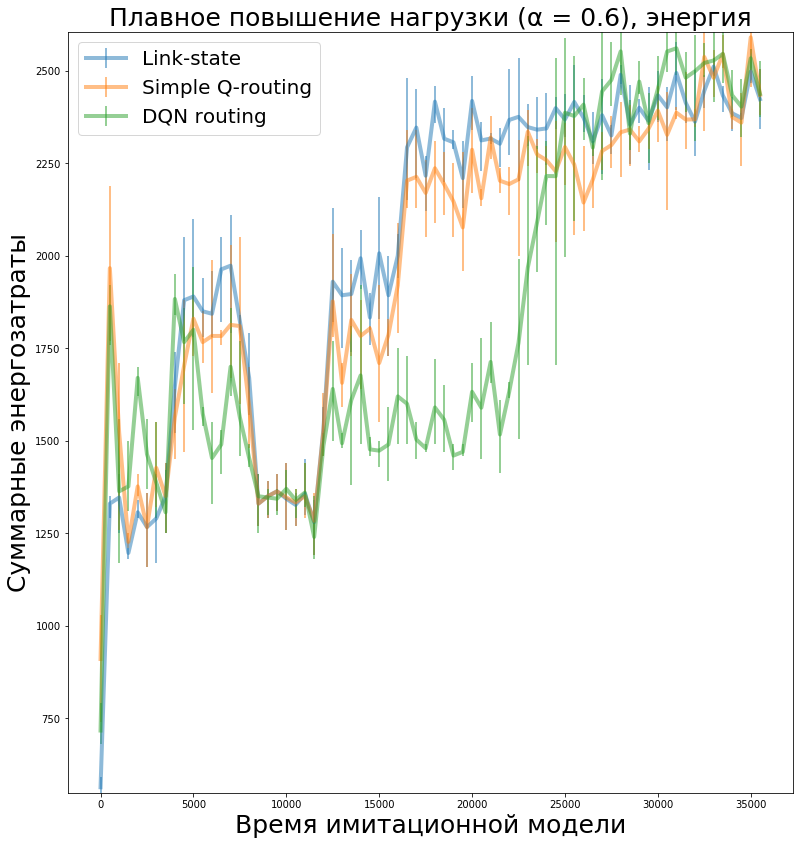
\includegraphics[width=\textwidth]{experiment-conveyors-a06-energy-tall}
    \end{column}
  \end{columns}
\end{frame}

%-------------------------------------------------------

\begin{frame}
  \frametitle{Итоги}
  \begin{itemize}
    \item Разработан алгоритм маршрутизации на основе мультиагентного обучения
      нейросетей с подкреплением -- \textit{DQN-routing}
    \item Сравнены три архитектуры нейросетей
    \item Алгоритм показал лучшее качество маршрутизации во время экспериментов
      по сравнению с link-state алгоритмом (доминирующее семейство алгоритмов в
      сетевом роутинге) и алгоритмом Q-routing (табличное обучение с
      подкреплением)
    \item Алгоритм продемонстрировал способность эффективной работы в условиях
      модели конвейерной системы с учетом энергопотребления.
  \end{itemize}
\end{frame}

\begin{frame}
  \begin{center}
    {\Huge Спасибо за внимание!}
  \end{center}
\end{frame}

%-------------------------------------------------------
\appendix

\begin{frame}
  \frametitle{Иллюстрация несходимости алгоритма к оптимуму без предобучения}
  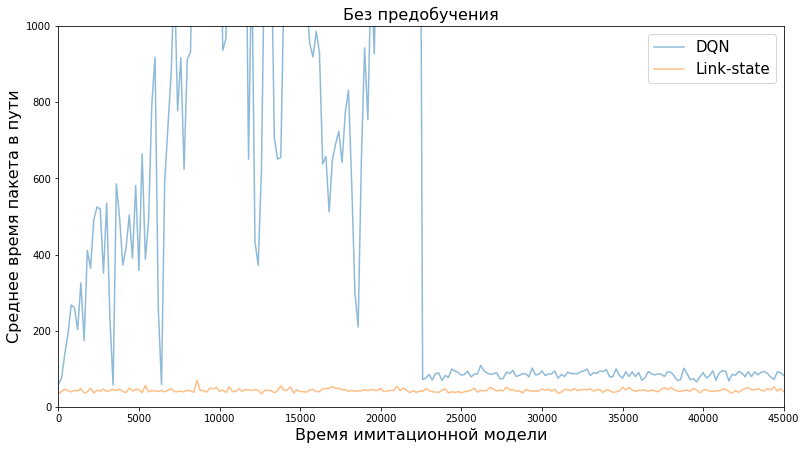
\includegraphics[width=\textwidth]{non-convergence}
\end{frame}

\begin{frame}
  \frametitle{Сравнение алгоритмов оптимизации: скорость предобучения}
  \begin{columns}
    \begin{column}{0.5\textwidth}
      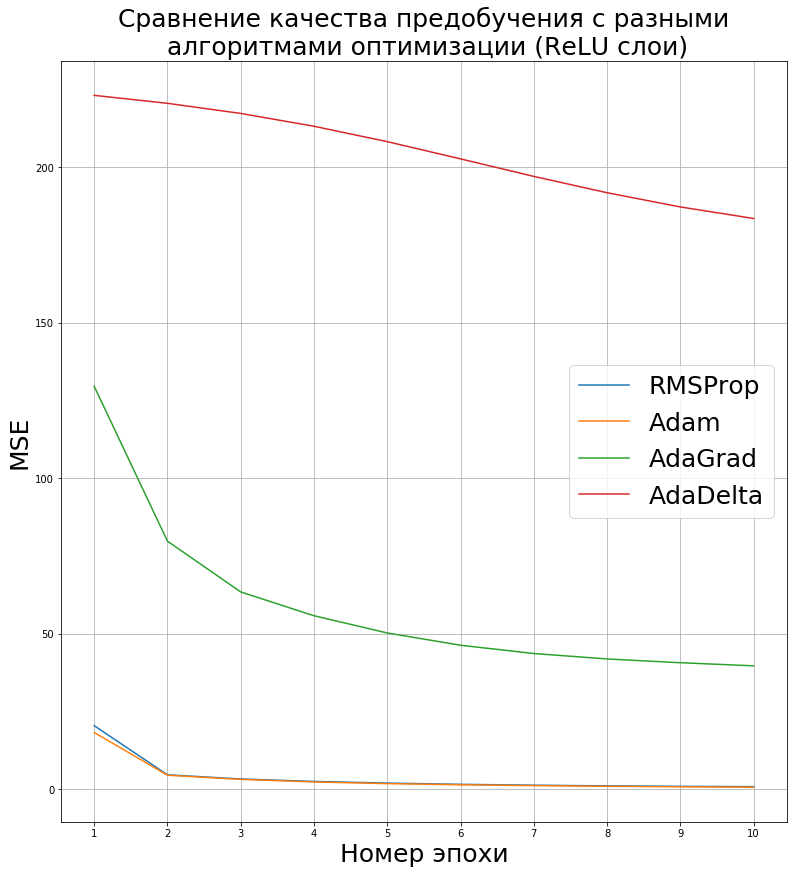
\includegraphics[width=\textwidth]{experiment-optimizers-pretrain-tall}
    \end{column}
    \begin{column}{0.5\textwidth}
      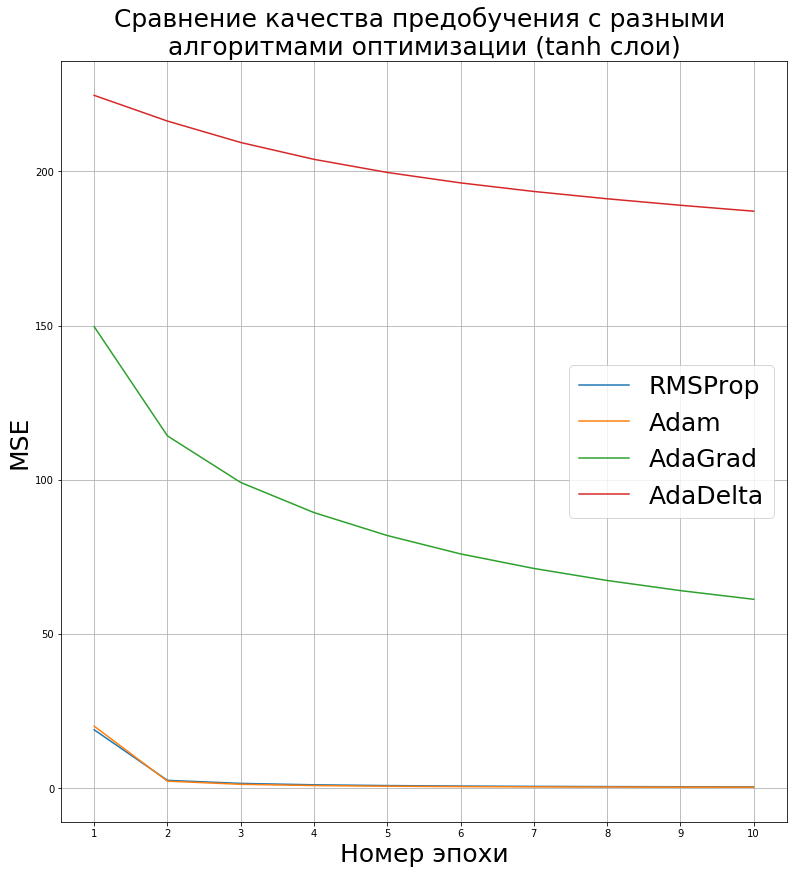
\includegraphics[width=\textwidth]{experiment-optimizers-pretrain-tanh-tall}
    \end{column}
  \end{columns}
\end{frame}

\begin{frame}
  \frametitle{Сравнение алгоритмов оптимизации и функций активации: скорость предобучения}
  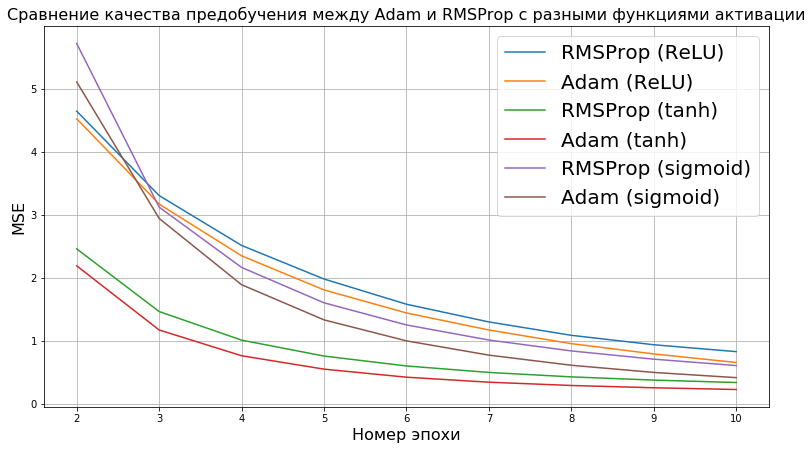
\includegraphics[width=\textwidth]{experiment-optimizers-pretrain-adam-vs-rmsprop}
\end{frame}

\begin{frame}
  \frametitle{Сравнение RMSProp и Adam в модели компьютерной сети}
  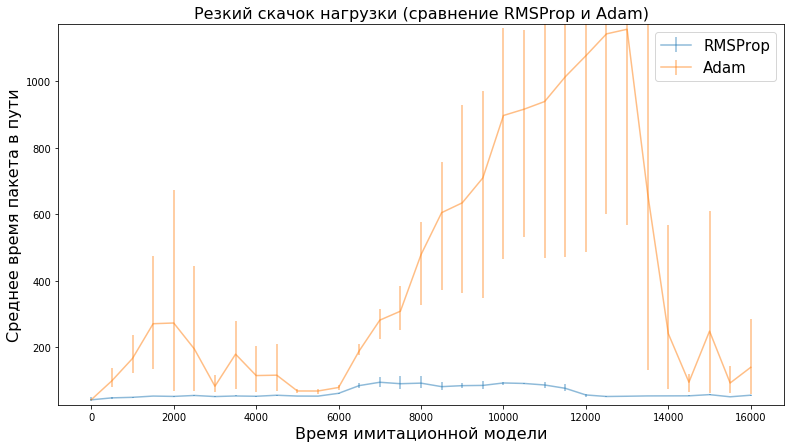
\includegraphics[width=\textwidth]{experiment-adam-failure}
\end{frame}

\begin{frame}
  \frametitle{Сравнение фукнций активации c RMSProp в модели компьютерной сети}
  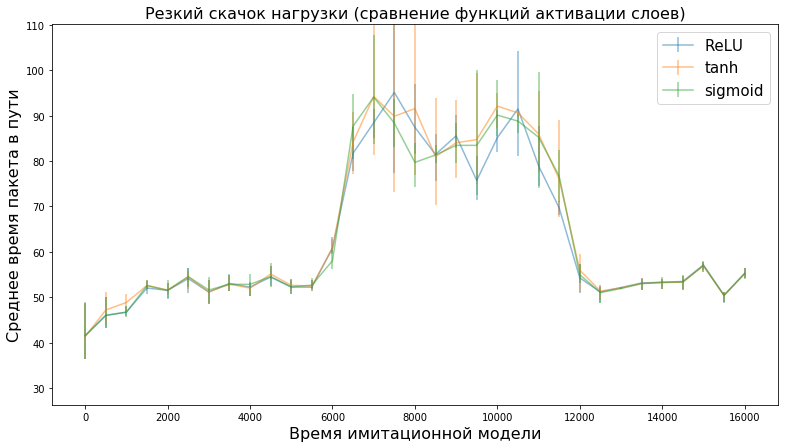
\includegraphics[width=\textwidth]{experiment-activations-launch}
\end{frame}

\begin{frame}
  \frametitle{Сравнение различных конфигураций feed-forward нейросети по
    качеству предобучения}
  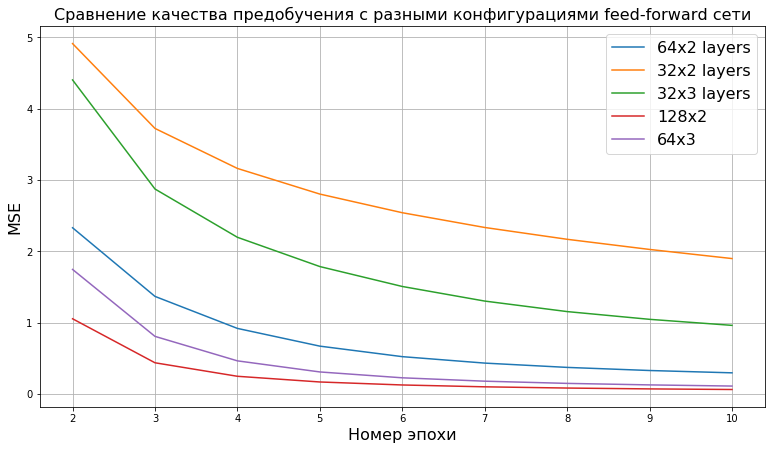
\includegraphics[width=\textwidth]{experiment-layers-pretrain}
\end{frame}

\begin{frame}
  \frametitle{Сравнение различных конфигураций feed-forward нейросети при работе
    в имитационной модели}
  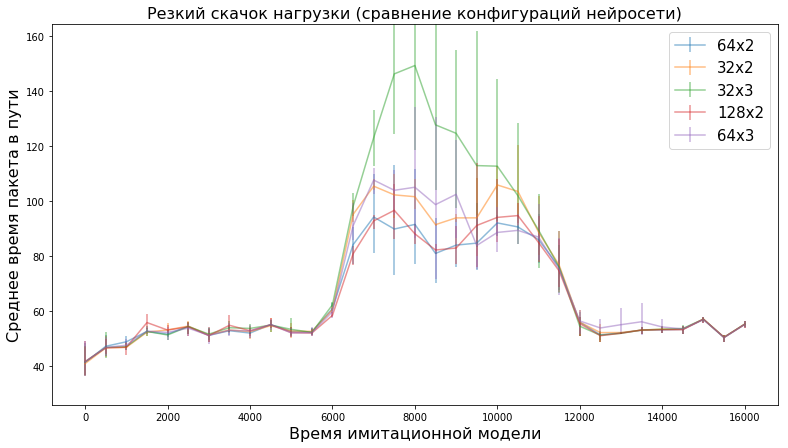
\includegraphics[width=\textwidth]{experiment-layers-launch}
\end{frame}

\begin{frame}
  \frametitle{Влияние softmax-стратегии на работу алгоритма}
  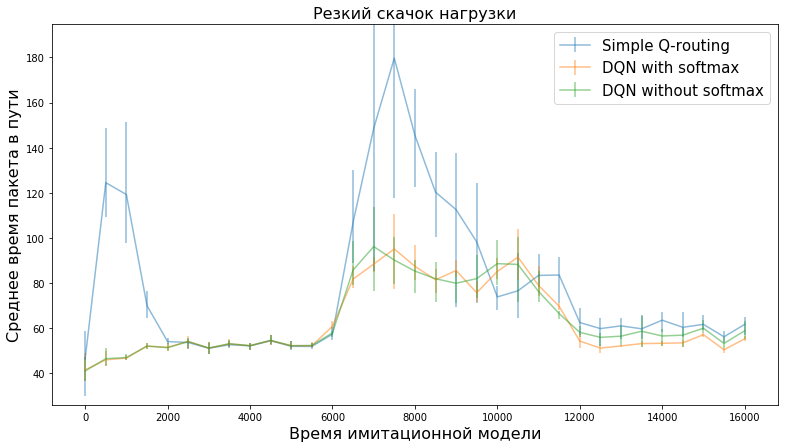
\includegraphics[width=\textwidth]{experiment-softmax-effect}
\end{frame}

\begin{frame}
  \frametitle{Влияние различных видов experience replay на работу алгоритма}
  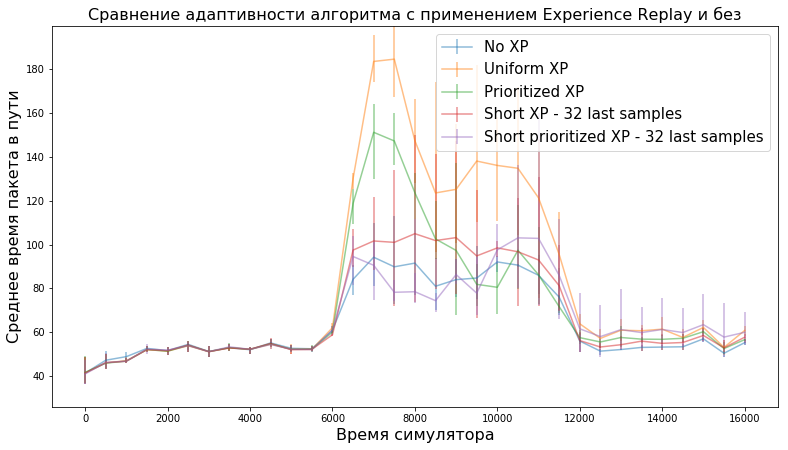
\includegraphics[width=\textwidth]{experiments-xp-variants}
\end{frame}

\begin{frame}
  \frametitle{Влияние включения матрицы смежности в наблюдаемое состояние}
  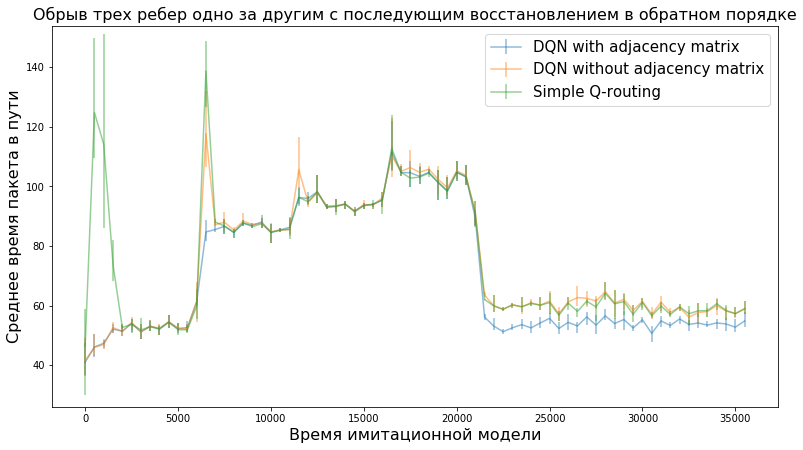
\includegraphics[width=\textwidth]{experiment-with-without-amatrix}
\end{frame}

\begin{frame}
  \frametitle{Влияние включения информации о состоянии соседних конвейеров в
    наблюдаемое состояние}
  \begin{columns}
    \begin{column}{0.5\textwidth}
      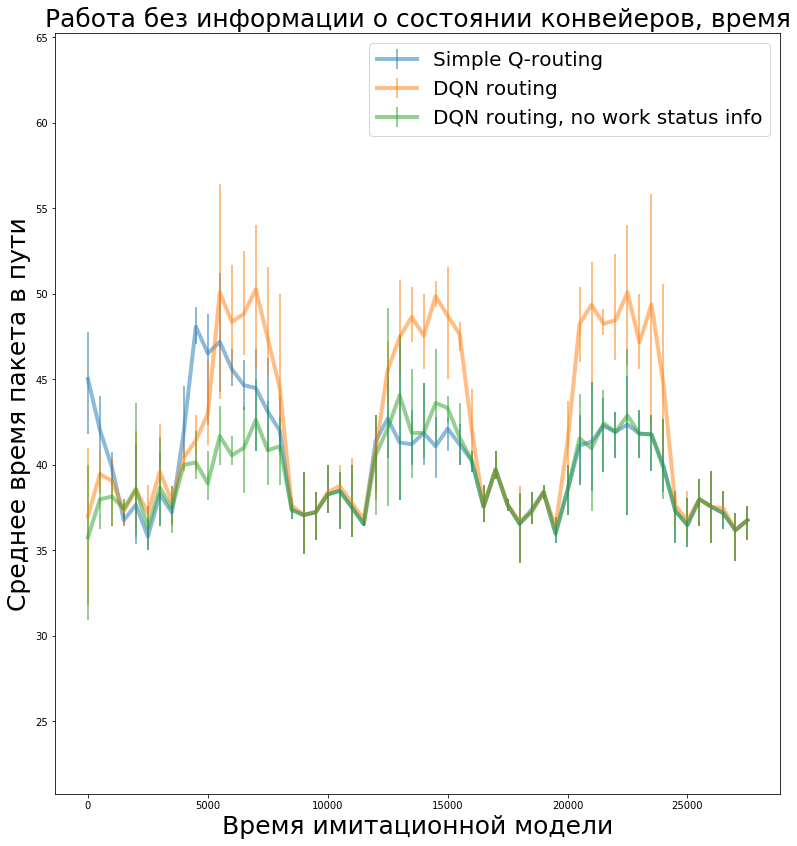
\includegraphics[width=\textwidth]{experiment-conveyors-en1-time-no-ws-tall}
    \end{column}
    \begin{column}{0.5\textwidth}
      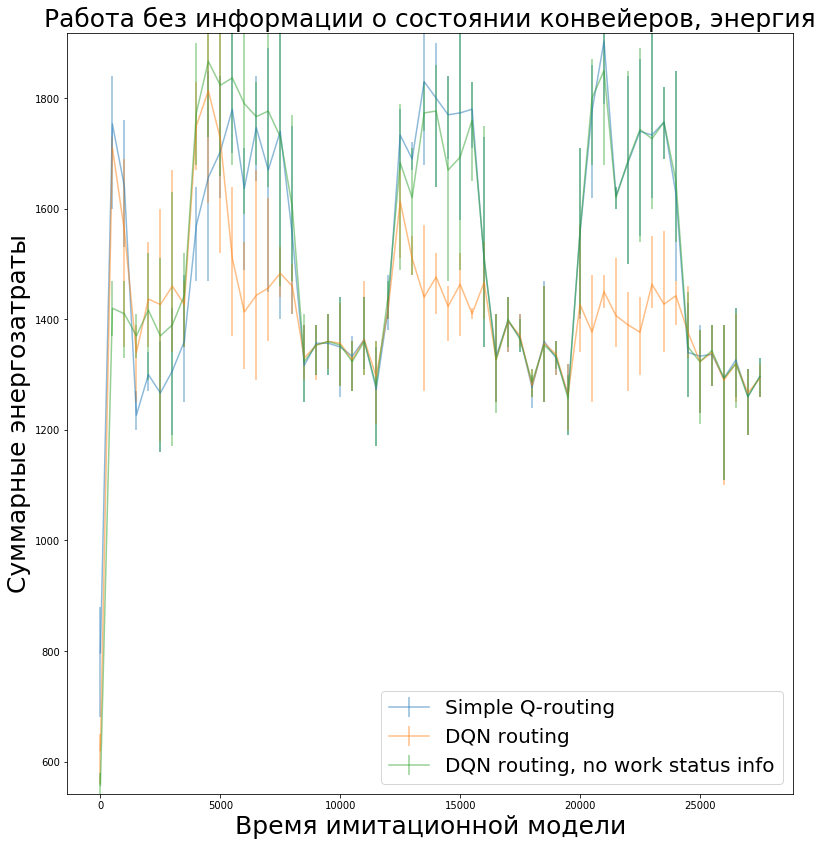
\includegraphics[width=\textwidth]{experiment-conveyors-en1-energy-no-ws-tall}
    \end{column}
  \end{columns}
\end{frame}

\end{document} 
